\documentclass[10pt]{article}
\usepackage[margin=1.05cm,top=0.8cm,bottom=0.8cm,columnsep=0.55cm]{geometry}
\usepackage[utf8]{inputenc}
\usepackage[T1]{fontenc}
\usepackage{lmodern}
\usepackage{microtype}
\usepackage{multicol}
\usepackage{booktabs}
\usepackage{xcolor}
\usepackage{hyperref}
\usepackage{tikz}
\usetikzlibrary{positioning,arrows.meta}

\definecolor{ucblue}{RGB}{0,51,102}
\hypersetup{colorlinks=true,urlcolor=ucblue,linkcolor=ucblue}
\setlength{\parindent}{0pt}
\setlength{\parskip}{2.5pt}
\pagestyle{empty}
\newcommand{\head}[1]{\textbf{\color{ucblue}#1}\hspace{0.4em}}
\newcommand{\VideoURL}{\textit{(video link pending)}}

\begin{document}

\begin{center}
{\Large\bfseries\color{ucblue} SQL4Business: Deliverable 2}\\[2pt]
{\small Generative Artificial Intelligence (580694), Universidad de Concepci\'on}\\[1pt]
{\small Aredhel Jim\'enez, Bryan Riquelme, Guido Salazar, Vicente So\~nez}\\[1pt]
{\small Code: \href{https://github.com/VicenteSonez/Asistente-SQL-4-Business}{github.com/VicenteSonez/Asistente-SQL-4-Business}
\quad$\vert$\quad Video: \VideoURL}
\end{center}

\vspace{-2pt}
\begin{center}
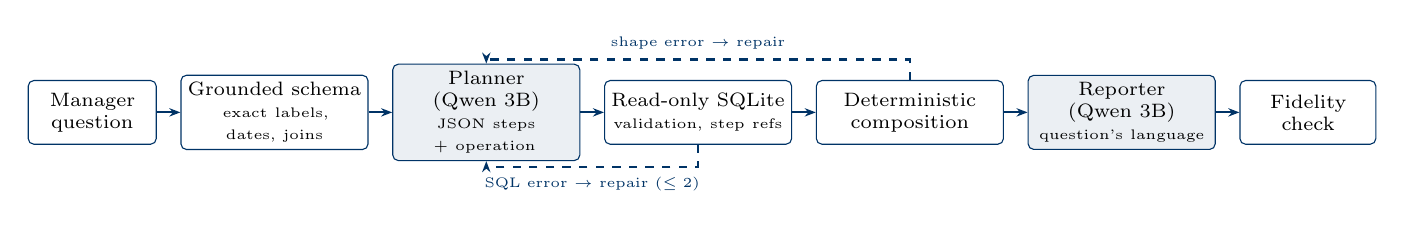
\begin{tikzpicture}[
  box/.style={draw=ucblue, rounded corners=2pt, align=center, font=\scriptsize, inner sep=2.5pt, minimum height=2.3em, text width=#1},
  box/.default=2.2cm,
  llm/.style={box=#1, fill=ucblue!8}, llm/.default=2.2cm,
  arrow/.style={-{Stealth[length=4pt]}, thick, ucblue}, node distance=0.3cm]
  \node[box=1.45cm] (q) {Manager\\question};
  \node[box, right=of q] (s) {Grounded schema\\{\tiny exact labels, dates, joins}};
  \node[llm, right=of s] (p) {Planner (Qwen 3B)\\{\tiny JSON steps + operation}};
  \node[box, right=of p] (x) {Read-only SQLite\\{\tiny validation, step refs}};
  \node[box, right=of x] (c) {Deterministic\\composition};
  \node[llm, right=of c] (r) {Reporter (Qwen 3B)\\{\tiny question's language}};
  \node[box=1.55cm, right=of r] (f) {Fidelity\\check};
  \foreach \a/\b in {q/s, s/p, p/x, x/c, c/r, r/f} \draw[arrow] (\a) -- (\b);
  \draw[arrow, dashed] (x.south) -- ++(0,-0.28) -| node[pos=0.25, below, font=\tiny] {SQL error $\rightarrow$ repair ($\leq 2$)} (p.south);
  \draw[arrow, dashed] (c.north) -- ++(0,0.26) -| node[pos=0.25, above, font=\tiny] {shape error $\rightarrow$ repair} (p.north);
\end{tikzpicture}
\end{center}
\vspace{-6pt}

\begin{multicols}{2}
\small

\head{Task, failure and model.} Unchanged from Deliverable 1: answer punctual and combined business
questions by executing the necessary SQL and reporting only figures faithful to the results. With
direct prompting, all three candidates scored 0/5 on combined questions (invented years,
translated labels, other SQL dialects, one query for a multi-value question). We commit to
\texttt{Qwen/Qwen2.5-Coder-3B-Instruct} (revision \texttt{488639f}, NF4 4-bit, bf16 compute, greedy
decoding, Colab T4): the smallest candidate, tied for the best local baseline (46.7\%);
Qwen-7B scored 33.3\% and Llama-8B also 46.7\% with more parameters and gated access.

\head{Intervention.} Each part targets a diagnosed error. The grounded schema lists exact labels,
the date range and join keys (translated labels, invented years). The planner decomposes the
question into SQL steps and names one operation; code, not the model, computes growth, share,
comparison and filter-then-rank (combined questions, mental arithmetic). SQLite runs read-only;
validation or shape errors go back to the planner up to twice. A later step may read an
earlier one (\texttt{FROM step\_1}), expanded as a CTE. The reporter writes in the question's
language, and the fidelity check accepts a figure only if it equals the verified answer or
the evidence at the precision written, and checks the stated direction of a change.

\head{Evaluation.} Official set: the 15 Deliverable 1 questions (10 punctual, 5 combined), used
while developing, so in-sample. Held-out set: 12 paraphrases (5/7) with the same gold, written
during an audit and not used for design. Every system gets the same inputs and criteria:
\textit{sql} is the Deliverable 1 criterion (each gold result set produced exactly);
\textit{answer} checks the final answer, however it was computed; \textit{report} and
\textit{e2e} (answer and report correct) apply to the solution. The baseline is the
Deliverable 1 prompt verbatim; the alternative strategy adds only the grounded schema to it.

\head{Results (table below).} The solution answers 11/15 official and 10/12 held-out
questions, against 8/15 and 5/12 for the baseline; on combined questions, 2/5 and 5/7
against 1/5 and 2/7. It answers and reports faithfully in 10/15 and 10/12. The grounded schema
alone gives most punctual gains (9/10 official answers); decomposition adds the combined ones.
Cost on the T4: 16.3\,s per question against 6.2\,s for the baseline.

\head{Declared deviations.} (1) The first version (17-09) chose the operation with keywords
copied from the 5 combined questions and vetoed other plans: 12/15 in-sample but 0/7 on
combined paraphrases. It was removed. (2) That version also used a new English baseline prompt
(40\%); the D1 prompt is restored. (3) The \textit{answer} metric was added because the
\textit{sql} criterion rejects correct one-query answers (the baseline answers q14 correctly).
(4) QLoRA fine-tuning, planned in D1, was not applied. (5) The first run of this version (v2)
discarded plain-text reports as malformed JSON; v3 changes only the reporter's output format,
and its SQL and answers are identical to v2 in 27/27 questions.

\head{Failure case: q09.} The planner filters \texttt{strftime('\%Y-\%m', sale\_date) BETWEEN
'2026-03-01' AND '2026-05-31'}. Comparing \texttt{'2026-03'} with a full date drops March and
June, so the code computes 70.06\% growth instead of 60.13\%. The SQL is valid, the result is
a single number and the report is faithful to it, so neither validation, repair nor the
fidelity check can see the error: they check form and figures, not the meaning of a predicate.
In q10 the model returns \texttt{strftime('\%Q')} again after the error message, and in q09-p
(held-out) it plans a single step, so the growth is never computed; its report invents 26\%,
10\% and 12\%, and the check rejects it.

\head{Limits.} Official results are in-sample and both sets are small (27 questions, synthetic
data). The fidelity check verifies figures, not their attribution: in q11 it accepts 488
reported as the total, and in q14-p a product id taken from a step. It is also conservative:
it rejects ``step 1'' in q13. When the planner picks \textit{direct} for a combined question,
the answer depends on one query. Retries rarely fix a plan (strong model priors).

\head{Reproduction.} \texttt{notebooks/deliverable2\_demo.ipynb} on a Colab T4 (\textit{Run all},
about 25 min) clones the repository, runs the demo shown in the video and the evaluation, and
writes \texttt{results/deliverable2\_v3.json} and the table below; no uploads or tokens needed.
\end{multicols}

\vspace{-4pt}
\begin{center}
\footnotesize
\begin{tabular}{@{}llccccc@{}}
\toprule
& & \multicolumn{3}{c}{\textbf{Official set (in-sample)}} & \multicolumn{2}{c}{\textbf{Held-out paraphrases}} \\
\cmidrule(lr){3-5}\cmidrule(l){6-7}
\textbf{System} & \textbf{Metric} & Punctual & Combined & All & Punctual & Combined \\
\midrule
Direct prompt (D1 baseline) & sql & 7/10 & 0/5 & 7/15 & 3/5 & 0/7 \\
 & answer & 7/10 & 1/5 & 8/15 & 3/5 & 2/7 \\
\addlinespace
Direct prompt + grounded schema & sql & 8/10 & 0/5 & 8/15 & 4/5 & 0/7 \\
 & answer & 9/10 & 1/5 & 10/15 & 4/5 & 4/7 \\
\addlinespace
Structured solution & sql & 9/10 & 2/5 & 11/15 & 5/5 & 3/7 \\
 & answer & 9/10 & 2/5 & 11/15 & 5/5 & 5/7 \\
 & report & 8/10 & 4/5 & 12/15 & 5/5 & 6/7 \\
 & e2e & 8/10 & 2/5 & 10/15 & 5/5 & 5/7 \\
\bottomrule
\end{tabular}

\end{center}

\end{document}
